\documentclass[12pt]{article}
\usepackage[utf8]{inputenc}
\usepackage[T1]{fontenc}
\usepackage{amsmath}
\usepackage{amsfonts}
\usepackage{amssymb}
\usepackage[version=4]{mhchem}
\usepackage{stmaryrd}
\usepackage{enumerate}% http://ctan.org/pkg/enumerate
\usepackage{titling}
\usepackage{pgfplots}
\usepackage{tikz}
\usepackage{graphicx}
\usepackage{caption}

\pretitle{\begin{center}\fontsize{18bp}{18bp}\selectfont}
    \posttitle{\par\end{center}}
\predate{\begin{center}\fontsize{14bp}{14bp}\selectfont}
    \postdate{\par\end{center}\vspace{24bp}}
\preauthor{}
\author{}
\postauthor{}

\setlength{\parindent}{0pt}

\title{Mathematical Methods II Assignment T1 }
\date{22 March, 2024}

\begin{document}

\maketitle
    \begin{itemize}
          \item Attempt all seven questions. There are 40 marks available.
          \item This assignment is open-book; you may use any resources at your disposal (calculator, graphing software, etc.), but the work you submit must be your own.
          \item You should write your solutions in detail, indicating which theorems or techniques you have applied and why they are valid. Solutions will be marked on their accuracy and validity as well as how clearly they are explained.
          \item Your grade for this assignment is worth $5 \%$ of your total grade.
          \item You may choose to handwrite and scan your solutions, type them, or a mixture of both.
          \item Your solutions must be uploaded to Canvas by 13:00 on Friday 22nd March.
        \end{itemize}
    \newpage
    
Biologists have discovered a new species of tropical bird, which they call a ladelbill. The new species looks very similar to an existing species of bird called a spoonbill. Ladelbills can only be distinguished from spoonbills because they usually have a longer wingspan.

The wingspan $Z$ of a ladelbill, in metres, is a random variable whose probability density function can be modelled by a normal distribution

$$
f(z)=\frac{1}{\sigma \sqrt{2 \pi}} e^{-(z-\mu)^{2} /\left(2 \sigma^{2}\right)}
$$

where $\mu$ is the mean wingspan, and $\sigma$ is the standard deviation: how spread out the values of $Z$ are.

This means that the probability a ladelbill has wingspan between $a$ and $b$ metres is $\int_{a}^{b} f(z) \mathrm{d} z$.

\section*{Question 1}
Write down your student number. It will look something like 230XXXXX. Write down the number $A=1.4 \mathrm{XX}$, where $\mathrm{XX}$ are the \textbf{final two digits} of your student number.

For example, if your student number is 23012345, your value for $A$ will be 1.445.

\subsection*{Q1 Answer}
Student Number: 02281337 \\
$A = 1.437$


\section*{Question 2}
Suppose the mean wingspan is $\mu=A$, and the standard deviation in wingspan is $\sigma=0.1$.
\begin{enumerate}[i.]
    \item Plot a graph of $f(z)$ for $z$ between 0.5 and 1.5. You may do this by hand or using graphing software, but in any case you should work out a table of values.
    \item Use calculus to work out the co-ordinates of the maxima and minima of the graph.
    \item Find $\lim _{z \rightarrow-\infty} f(z)$ and $\lim _{z \rightarrow \infty} f(z)$. How do you interpret these values in the context of probability?
\end{enumerate}

\subsection*{Q2 Answer}
\begin{enumerate}[i.]
    \item
    $$
    f(z) = \frac{1}{\sigma \sqrt{2 \pi}} e^{-(z-\mu)^{2} /\left(2 \sigma^{2}\right)}
    \text{ where } \mu = A = 1.437 \text{ and } \sigma = 0.1
    $$
    Thus
    $$
    f(z) = \frac{1}{(0.1) \cdot \sqrt{2 \pi}} e^{-(z-(1.437))^{2} /\left(2 \cdot (0.1)^{2}\right)}
    $$
    Graph and Table:
    \newline
    
    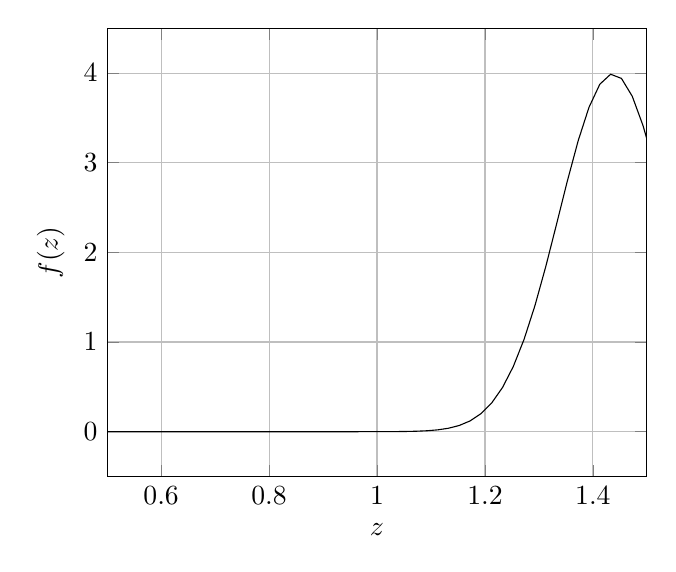
\begin{tikzpicture}
        \begin{axis}[ 
          xlabel=$z$,
          ylabel={$f(z)$},
          xmin = 0.5,
          xmax = 1.5,
          ymin = -0.5,
          ymax = 4.5,
          % axis x line = middle,
          % axis y line = middle,
          no markers, grid
        ] 
          \addplot [black, samples = 500]{(1/(0.1*sqrt(2*pi))*e^(-(x-1.437)^2 / (2*0.1^2)}; 
        \end{axis}
    \end{tikzpicture}
    \newline
    
    \begin{tabular}{c|c}
           z& f(z)\\ \hline
           0.5 & 3.436 $\cdot 10^{-19}$\\
           0.7 & 6.399 $\cdot 10^{-12}$\\
           0.9& 2.183 $\cdot 10^{-6}$\\
           1.1& 1.364 $\cdot 10^{-2}$\\
           1.3& 1.561 \\
           1.5& 3.271
    \end{tabular}{}
    \newline
    \item In order to find the maxima and minima, we need to find the first and second derivatives of $f(z)$. \newline
    \textbf{First Derivative:}
    \begin{equation}
        f'(z) = \frac{d}{dz}[f(z)] = \frac{d}{dz}[\frac{1}{(0.1) \cdot \sqrt{2 \pi}} e^{-(z-(1.437))^{2} /\left(2 \cdot (0.1)^{2}\right)}]
    \end{equation}
    simplify the expression:
    \begin{equation}
        f'(z) = \frac{d}{dz} \left [\frac{5 \sqrt{2} \cdot e^{-50(z-\frac{1437}{1000})^2}}{\sqrt{\pi}} \right ]
    \end{equation}
    pull out the constant: \\
    $[a \cdot u(x) + b*v(x)]' = a*u'(x) + b*v'(x)$
    \begin{equation}
        f'(z) = \frac{5 \sqrt{2}}{\sqrt{\pi}} \cdot \frac{d}{dz} \left [e^{-50(z-\frac{1437}{1000})^2} \right ]
    \end{equation}
    apply the exponential function rule: \\
    $[e^u(x)]' = u'(x) * e^u(x)$
    \begin{equation}
        \begin{aligned}
            f'(z) = {}
            & \left (\frac{5 \sqrt{2}}{\sqrt{\pi}} \right ) \cdot \left (e^{-50(z-\frac{1437}{1000})^2} \right ) \\
            & \cdot \left ( -50 \cdot \frac{d}{dz} \left [\left (z-\frac{1437}{1000} \right )^2 \right ] \right )
        \end{aligned}
    \end{equation}
    apply the chain and power rules: \\
    Chain Rule: $[u(v(x))] = u'(v(x)) * v'(x)$ \\
    Power Rule: $[u(x)^n]' = n*u(x)^{n-1} * u'(x)$ \\
    \begin{equation}
        \begin{aligned}
            f'(z) = {}
            & \left (\frac{5 \sqrt{2}}{\sqrt{\pi}} \right ) \cdot \left (e^{-50(z-\frac{1437}{1000})^2} \right ) \\
            & \cdot \left ( -50 \cdot 2 \left (z - \frac{1437}{1000} \right ) \cdot \frac{d}{dz} \left [z-\frac{1437}{1000} \right ] \right )
        \end{aligned}
    \end{equation}
    pull out constant factors: \\
    $[a*u(x)]' = a*u'(x)$
    \begin{equation}
        \begin{aligned}
            f'(z) = {}
            & \left (\frac{5 \sqrt{2}}{\sqrt{\pi}} \right ) \cdot \left (e^{-50(z-\frac{1437}{1000})^2} \right ) \\
            & \cdot \left ( -50 \cdot 2 \left (z - \frac{1437}{1000} \right ) \cdot \left (\frac{d}{dz} \left [z \right ] + \frac{d}{dz} \left [\frac{1437}{1000} \right ] \right ) \right )
        \end{aligned}
    \end{equation}
    power rule: \\
    $[u(x)^n]' = n*u(x)^{n-1} * u'(x)$
    \begin{equation}
        f'(z) = \left (\frac{5 \sqrt{2}}{\sqrt{\pi}} \right ) \cdot \left (e^{-50(z-\frac{1437}{1000})^2} \right ) \cdot \left ( -50 \cdot 2 \left (z - \frac{1437}{1000} \right ) \cdot \left (1+0 \right ) \right )
    \end{equation}
    simplify the expression:
    \begin{equation}
        f'(z) = - \frac{125 \cdot 2^{\frac{5}{2}} \left ( z - \frac{1437}{1000}\right ) e^{-50\left (z-\frac{1437}{1000} \right )^2}}{\sqrt{\pi}}
    \end{equation}
    \begin{equation}
        f'(z) = - \frac{(1000z - 1437)e^{-50 \left (z-\frac{1437}{1000} \right )^2}}{\sqrt{2}\sqrt{\pi}}
    \end{equation}
    \setcounter{equation}{0}
    \textbf{Second Derivative:}
    \begin{equation}
        f''(z) = \frac{d}{dz}[f'(z)] = \frac{d}{dz} \left [- \frac{(1000z - 1437)e^{-50 \left (z-\frac{1437}{1000} \right )^2}}{\sqrt{2}\sqrt{\pi}} \right ]
    \end{equation}
    pull out the constants: \\
    $[a*u(x)]' = a*u'(x)$
    \begin{equation}
        f''(z) = - \frac{1}{\sqrt{2}\sqrt{\pi}} \cdot \frac{d}{dz} \left [(1000z - 1437)e^{-50 \left (z-\frac{1437}{1000} \right )^2} \right ]
    \end{equation}
    apply the product rule: \\
    $[u(x)*v(x)]' = u'(x)*v(x) + u(x)*v'(x)$
    \begin{equation}
        \begin{aligned}
            f''(z) = {}
            & - \frac{1}{\sqrt{2}\sqrt{\pi}} \cdot (\frac{d}{dz} \left [1000z - 1437 \right ] \cdot e^{-50 \left (z-\frac{1437}{1000} \right )^2} \\
            & + (1000z - 1437) \cdot \frac{d}{dz} \left [e^{-50 \left (z-\frac{1437}{1000} \right )^2} \right ] )
        \end{aligned}
    \end{equation}
    pull out constants and apply exponential function rule: \\
    pull out constants: $[a*u(x)]' = a*u'(x)$ \\
    exponential function rule: $[e^u(x)]' = u'(x) * e^u(x)$ \\
    \begin{equation}
        \begin{aligned}
            f''(z) = {}
            & - \frac{1}{\sqrt{2}\sqrt{\pi}} \cdot ((1000 \cdot \frac{d}{dz} \left [z \right ] + \frac{d}{dz} \left [-1437 \right ])e^{-50 \left (z-\frac{1437}{1000} \right )^2} \\
            & + (1000z - 1437)e^{-50 \left (z-\frac{1437}{1000} \right )^2} \cdot \frac{d}{dz} \left [-50 \left (z-\frac{1437}{1000} \right )^2 \right ] )
        \end{aligned}
    \end{equation}
    pull out constants and apply power rule: \\
    pull out constants: $[a*u(x)]' = a*u'(x)$ \\
    power rule: $[u(x)^n]' = n*u(x)^{n-1} * u'(x)$ \\
    \begin{equation}
        \begin{aligned}
            f''(z) = {}
            & - \frac{1}{\sqrt{2}\sqrt{\pi}} \cdot ((1000 \cdot 1 + 0)e^{-50 \left (z-\frac{1437}{1000} \right )^2} \\
            & + (1000z - 1437)e^{-50 \left (z-\frac{1437}{1000} \right )^2} \\
            & \cdot \left (-50 \cdot \frac{d}{dz} \left [ \left (z-\frac{1437}{1000} \right )^2 \right ] \right ) )
        \end{aligned}
    \end{equation}
    apply power rule: \\
    power rule: $[u(x)^n]' = n*u(x)^{n-1} * u'(x)$ \\
    \begin{equation}
        \begin{aligned}
            f''(z) = {}
            & - \frac{1}{\sqrt{2}\sqrt{\pi}} \cdot (1000e^{-50 \left (z-\frac{1437}{1000} \right )^2} \\
            & -50(1000z - 1437)e^{-50 \left (z-\frac{1437}{1000} \right )^2} \\
            & \cdot 2 \left (z-\frac{1437}{1000} \right ) \cdot \frac{d}{dz} \left [ \left (z-\frac{1437}{1000} \right ) \right ] )
        \end{aligned}
    \end{equation}
    pull out constants: \\
    pull out constants: $[a*u(x)]' = a*u'(x)$ \\
    \begin{equation}
        \begin{aligned}
            f''(z) = {}
            & - \frac{1}{\sqrt{2}\sqrt{\pi}} \cdot (1000e^{-50 \left (z-\frac{1437}{1000} \right )^2} \\
            & -100(1000z - 1437)e^{-50 \left (z-\frac{1437}{1000} \right )^2} \\
            & \cdot \left (z-\frac{1437}{1000} \right ) \left (\frac{d}{dz} \left [ z \right ] + \frac{d}{dz} \left [ - \frac{1437}{1000} \right ]\right ) )
        \end{aligned}
    \end{equation}
    apply power rule: \\
    power rule: $[u(x)^n]' = n*u(x)^{n-1} * u'(x)$ \\
    \begin{equation}
        \begin{aligned}
            f''(z) = {}
            & - \frac{1}{\sqrt{2}\sqrt{\pi}} \cdot (1000e^{-50 \left (z-\frac{1437}{1000} \right )^2} \\
            & -100(1000z - 1437)e^{-50 \left (z-\frac{1437}{1000} \right )^2} \\
            & \cdot \left (z-\frac{1437}{1000} \right ) \left (1+0\right ) )
        \end{aligned}
    \end{equation}
    simplify the expression:
    \begin{equation}
        \begin{aligned}
            f''(z) = {}
            & - \frac{1}{\sqrt{2}\sqrt{\pi}} \cdot (1000e^{-50 \left (z-\frac{1437}{1000} \right )^2} \\
            & -100\left (z-\frac{1437}{1000} \right )(1000z - 1437) \\
            & \cdot e^{-50 \left (z-\frac{1437}{1000} \right )^2} )
        \end{aligned}
    \end{equation}
    simplify the expression:
    \begin{equation}
        \begin{aligned}
            f''(z) = {}
            & \frac{(1000000z^2 - 2874000z +2054969)e^{-50 \left (z - \frac{1437}{1000} \right )^2}}{5 \cdot 2^{\frac{3}{2}} \sqrt{\pi}}
    \end{aligned}




    
    

    
\end{enumerate}

\section*{Question 3}
Use the Trapezium Rule with a suitable number of intervals to estimate the probability that a ladelbill has wingspan between 1.1 and 1.2 metres.

\section*{Question 4}
Use the Trapezium Rule Error Approximation to estimate the error in your approximation from Question 3.

The biologists have made some more observations, and conclude that the mean wingspan of a ladelbill is actually $\mu=1.6$ metres, with standard deviation $\sigma=0.1$.

\section*{Question 5}
How will this new observation affect the probability you worked out in Question 3?

\section*{Question 6}
The mean wingspan of a spoonbill is $\mu_{\text {spoon }}=1.2$ metres, with standard deviation $\sigma_{\text {spoon }}=0.1$.

\textbf{By transforming your graph from Question 2}, sketch a new graph of the probability density function of spoonbill wingspan.

\section*{Question 7}
The biologists observe a bird in the wild which could be a ladelbill or a spoonbill. It has wingspan of 1.15 metres. Discuss which species you think the bird is likely to be, making reference to your answers from Questions 2-6.


\end{document}